   
\documentclass[11pt, answers]{exam}
\renewcommand{\baselinestretch}{1.05}
\usepackage{amsmath,amsthm,verbatim,amssymb,amsfonts,amscd, graphicx}
\usepackage{graphics}

\usepackage{afterpage}
\usepackage{caption}

\usepackage{tikz}
\usepackage{fancybox}

\usepackage{clrscode3e}

\topmargin0.0cm
\headheight0.0cm
\headsep0.0cm
\oddsidemargin0.0cm
\textheight23.0cm
\textwidth16.5cm
\footskip1.0cm
\theoremstyle{plain}
\newtheorem{theorem}{Theorem}
\newtheorem{corollary}{Corollary}
\newtheorem{lemma}{Lemma}
\newtheorem{proposition}{Proposition}
\newtheorem*{surfacecor}{Corollary 1}
\newtheorem{conjecture}{Conjecture}  
\theoremstyle{definition}
\newtheorem{definition}{Definition}

 \begin{document}
 


\title{CSC265: Assignment 1}
\date{October 4th, 2016}
\author{Caroline (Ruo yi) Lin, written solution \\ Junjie Cheng, proofreading and revision}
\maketitle

\unframedsolutions

\begin{questions}

\question

\begin{parts}

\part Describe in detail a data structure implementing the Partial-Sums ADT. Draw an example with $n=8$, and values $a_1,\ldots,a_8$ of your choosing, but not $a_1=\ldots=a_8=0$. \\

\begin{solution}
The correct data structure is a full binary tree of height $k, B_k$. There are $2^k = n$ leaves in the lowest row of this tree. The $i$th leaf holds value $a_i$. The values of the parent nodes are defined recursively as the sum of their two children. An example is below with $a_1, \ldots, a_n = 1, 2, 3, 4, 5, 6, 7, 0$.
\\


\begin{center}
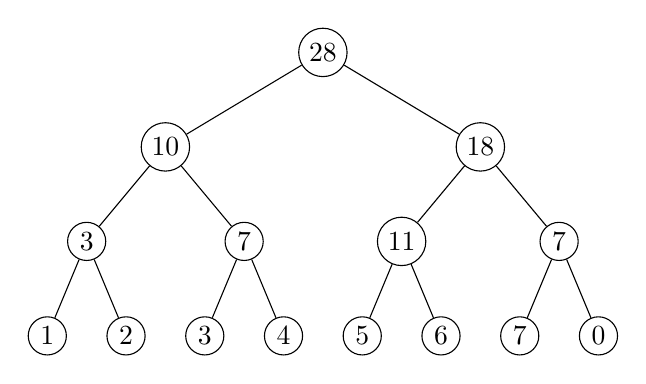
\begin{tikzpicture} 
[ 
level distance=12mm, 
every node/.style={circle, draw, inner sep=2pt},
level 1/.style={sibling distance=40mm}, 
level 2/.style={sibling distance=20mm}, 
level 3/.style={sibling distance=10mm}
]

\node {28} 
child {node {10} 
	child {node {3} 
		child {node {1}} 
		child {node {2}}
	}
	child {node {7} 
		child {node {3}} 
		child {node {4}}
	} 
}
child {node {18}
 	child {node {11} 
 		child {node {5}} 
 		child {node {6}}
 	}
 	child {node {7}
		child {node {7}}
		child {node {0}}
	}
};	 
\end{tikzpicture}
\end{center}

\end{solution}

\part Describe in clear and precise English how to implement the three operations $\proc{Init}$, $\proc{Add}(i,t)$, and $\proc{Sum}(i)$. Give pseudocode for $\proc{Add}(i,t)$, and $\proc{Sum}(i)$. For each operation argue why it computes the correct output, and show that it runs in the required worst-case running time.

\begin{itemize}
\item $\proc{Init}$ must run in time $\func{O}(n)$
\item $\proc{Add}(i,t)$ must run in time $\func{O}(\log(n))$
\item $\proc{Sum}(i)$ must run in time $\func{O}(\log(n))$
\end{itemize}

\begin{solution}\\

$\proc{Init}$:
Since $n = 2^k$, the binary tree required by the Partial-Sums ADT will always be full. Then the tree can be easily implemented as an array of size $2^{k+1} - 1$, with initial values all set to $0$. We assume that the first index of the array is $1$.

There is no need to construct pointers, since for a complete binary tree there are simple closed-form expressions for parent and child nodes. The functions are reproduced from CLRS Section 6.1.

Then $\proc{Init}$ runs in time $\func{O}(2^{k+1} - 1) = \func{O}(2(2^k)) = \func{O}(2n) = \func{O}(n)$.

\begin{codebox}
\Procname{$ \proc{Parent}(i)$}
\li 		\Return $\lfloor i/2 \rfloor$
\end{codebox}

\begin{codebox}
\Procname{$ \proc{Left-Child}(i)$}
\li 		\Return $2i$
\end{codebox}

\begin{codebox}
\Procname{$ \proc{Right-Child}(i)$}
\li 		\Return $2i + 1$
\end{codebox}

$\proc{Add}(i,t)$:
Add is simple to implement. The $i$th leaf of the tree is given by index $2^k + i$. We add $t$ to this leaf, and then add $t$ to each of $i$'s parents, grandparents, great-grandparents $\ldots$ until we reach the root.

\begin{codebox}
\Procname{$\proc{Add}(i,t)$}
\li $\func{node\_index} \gets 2^k + (i - 1)$
\li \While $\func{node\_index} \neq 0$
\li \Do $\func{node\_index.value} \gets \func{node\_index.value} + t$
\li $\func{node\_index} = \proc{Parent}(\func{node\_index})$
\End
\end{codebox}

The resultant tree has an updated leaf and satisfies the sum property specified in Q1(a). This is because only the parents of the leaf specified by $i$ will have their values affected.

$\proc{Add}(i,t)$ runs in $\func{O}(\log(n))$. One iteration of the while loop is executed for each level of the tree, so the algorithm is proportional to the tree height. This in turn is proportional to the log of the number of nodes in the tree, which is proportional to the number of leaves. \\

We may reach the same conclusion by noticing that $\func{node\_index}$ is proportional to $n$ and that it is halved on each iteration when $\proc{Parent}$ is called. It takes $\lfloor \log(n) \rfloor + 1$ iterations of the loop for $\func{node\_index}$ to reach zero.
\\

$\proc{Sum}(i)$:
Notice that for any node $N$ at depth $h$ of the tree, there are $2^{n-h}$ descendants of $N$ which are leaves. By induction, the value of $N$ is equal to the sum of its leaf descendants. 

This is key to our algorithm, because we can decompose the sum $\sum_{j=1}^{i}a_j$ into a sum of groups of powers of two. This binary representation of $i$ is unique.

For example, if $i=7$ and $n=2^3=8$, we may write $\sum_{j=1}^{i}a_j$ as $\sum_{j=1}^{2^2}a_j +\sum_{j=2^2 + 1}^{2^2 + 2^1}a_j + \sum_{j=2^2 + 2^1 + 1}^{2^2 + 2^1 + 2^0}a_j$. This first sum is a group of 4, the second a group of 2, and the third a group of 1. Now since each node at level $h$ of our tree corresponds to a group of $2^{k-h}$ leaf terms, we may choose nodes from levels 1, 2, and 3 respectively to represent these terms.

The resulting pseudocode is difficult to parse, so we also illustrate the procedure graphically below. 

\begin{minipage}[t]{\linewidth}
                \centering
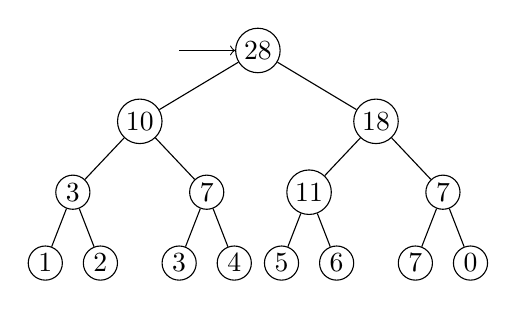
\begin{tikzpicture}
[ 
level distance=9mm, 
every node/.style={circle, draw, inner sep=1.5pt},
level 1/.style={sibling distance=30mm}, 
level 2/.style={sibling distance=17mm}, 
level 3/.style={sibling distance=7mm}
]

\node (root) {28} 
child {node {10} 
	child {node {3} 
		child {node {1}} 
		child {node {2}}
	}
	child {node {7} 
		child {node {3}} 
		child {node {4}}
	} 
}
child {node {18}
 	child {node {11} 
 		child {node {5}} 
 		child {node {6}}
 	}
 	child {node {7}
		child {node {7}}
		child {node {0}}
	}
};
\coordinate[left of=root] (invisi);
\draw[->] (invisi) -- (root);
\end{tikzpicture}
\end{minipage}

\begin{minipage}[t]{\linewidth}
                \centering
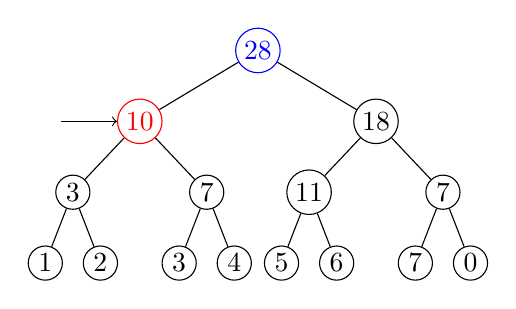
\begin{tikzpicture}
[ 
level distance=9mm, 
every node/.style={circle, draw, inner sep=1.5pt},
level 1/.style={sibling distance=30mm}, 
level 2/.style={sibling distance=17mm}, 
level 3/.style={sibling distance=7mm}
]

\node[blue] (root) {28} 
child {node[red] (hey) {10} 
	child {node {3} 
		child {node {1}} 
		child {node {2}}
	}
	child {node {7} 
		child {node {3}} 
		child {node {4}}
	} 
}
child {node {18}
 	child {node {11} 
 		child {node {5}} 
 		child {node {6}}
 	}
 	child {node {7}
		child {node {7}}
		child {node {0}}
	}
};
\coordinate[left of=hey] (invisi);
\draw[->] (invisi) -- (hey);
\end{tikzpicture}
\end{minipage}

\begin{minipage}[t]{\linewidth}
                \centering
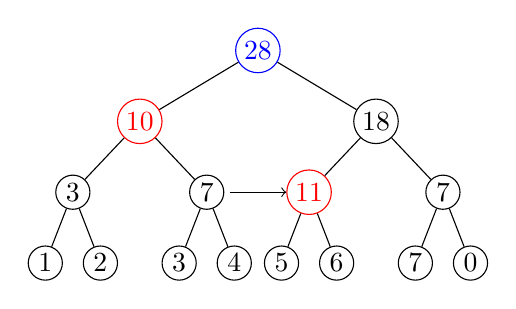
\begin{tikzpicture}
[ 
level distance=9mm, 
every node/.style={circle, draw, inner sep=1.5pt},
level 1/.style={sibling distance=30mm}, 
level 2/.style={sibling distance=17mm}, 
level 3/.style={sibling distance=7mm}
]

\node[blue] (root) {28} 
child {node[red] (hey) {10} 
	child {node {3} 
		child {node {1}} 
		child {node {2}}
	}
	child {node {7} 
		child {node {3}} 
		child {node {4}}
	} 
}
child {node {18}
 	child {node[red] (hey2) {11} 
 		child {node {5}} 
 		child {node {6}}
 	}
 	child {node {7}
		child {node {7}}
		child {node {0}}
	}
};
\coordinate[left of=hey2] (invisi);
\draw[->] (invisi) -- (hey2);
\end{tikzpicture}
\end{minipage}

\begin{minipage}[t]{\linewidth}
                \centering
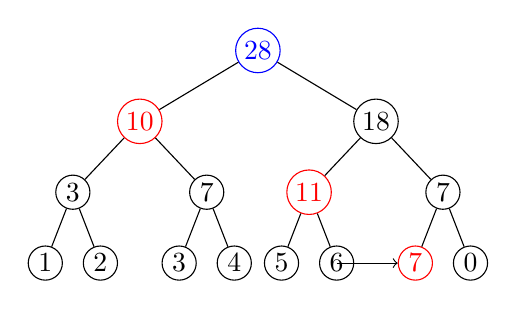
\begin{tikzpicture}
[ 
level distance=9mm, 
every node/.style={circle, draw, inner sep=1.5pt},
level 1/.style={sibling distance=30mm}, 
level 2/.style={sibling distance=17mm}, 
level 3/.style={sibling distance=7mm}
]

\node[blue] (root) {28} 
child {node[red] (hey) {10} 
	child {node {3} 
		child {node {1}} 
		child {node {2}}
	}
	child {node {7} 
		child {node {3}} 
		child {node {4}}
	} 
}
child {node {18}
 	child {node[red] (hey2) {11} 
 		child {node {5}} 
 		child {node {6}}
 	}
 	child {node {7}
		child {node[red] (hey3) {7}}
		child {node {0}}
	}
};
\coordinate[left of=hey3] (invisi);
\draw[->] (invisi) -- (hey3);
\end{tikzpicture}

\captionof{figure}{Procedure $\proc{Sum}(i)$ on the tree in Q1(a) with $i=7$. The procedure begins at the root of top of the tree. The arrow represents the node being considered. If the node is red, it is added to the running sum $x$. If it is blue, it has been visited but has not been added. }

\end{minipage}


\begin{codebox}
\Procname{$\proc{Sum}(i)$}
\li $d \gets 1$
\li $b \gets i$
\li $c \gets n$
\li $x \gets 0$
\li \While $b > 0$ \Do
\li		\If $(\lfloor b / c \rfloor = 1)$ \Then
\li 		$b \gets b - c$
\li			$x \gets x + \func{value}(d)$
\li 		$d = 2d + 2$
\li		\Else
\li			$d = 2d$	
		\End
\li	$c \gets \lfloor c / 2 \rfloor$ 		
	\End
\li \Return $x$
\end{codebox}

Note $\func{value}(d)$ is a function which returns the value of the node with index $d$. Intuitively, $b$ and $c$ are helper variables that decompose $i$ into a sum of powers of two, while $d$ holds the index of the next node to be visited by the algorithm, and $x$ holds the running sum of nodes visited so far.\\

\textit{Proof of Correctness.}\\
We will begin by proving a lemma which essentially states that the value held by a node is equal to the sum of the values of its leaf descendants.\\
\begin{lemma}
If the index of a node $d$ in an array-implementation of the Sum-ADT binary tree of height $k$ is $2^h + \mathit{l}$, then $\func{value}(d)$ is equal to \[\sum_{j = (2^{k-h})\mathit{l} + 1}^{(2^{k-h})\mathit{l} + 2^{k-h}}a_j.\]
\end{lemma}
\begin{proof}
We fix the size of the tree, $k$, and proceed by induction up the levels of the tree. 

\emph{Base case:} $h = k$. Fix $\mathit{l}$. Then $d$ is a leaf and 

\begin{gather*}
\sum_{j = (2^{k-h})\mathit{l} + 1}^{(2^{k-h})\mathit{l} + 2^{k-h}}a_j 
 = \sum_{j = \mathit{l} + 1}^{\mathit{l} + 1}a_j
 = a_{l + 1} = \func{value}(d)
\end{gather*}

So the base case holds. Note $\mathit{l} = 0$ for the first node at depth $h$ in the tree.

\emph{Inductive Case:} Suppose that the lemma holds for all nodes at depth $h + 1$ of the tree. We show that it holds for nodes at depth $h$. 

Fix $\mathit{l}$. By construction,  $\func{value}(d)$ is equal to the sum of the values of its left and right children. The index of the left child is $2(2^h + \mathit{l}) = 2^{h+1} + 2\mathit{l}$ and the index of the right child is $2(2^h + \mathit{l}) + 1 = 2^{h+1} + 2\mathit{l} + 1$. We apply the induction hypothesis on the children of $d$ to obtain

\begin{align*}
\func{value}(d) &= 
\sum_{j = (2^{k-(h+1)})(2 \mathit{l}) + 1}^{(2^{k-(h+1)})(2 \mathit{l}) + 2^{k-(h+1)}}a_j + 
\sum_{j = (2^{k-(h+1)})(2 \mathit{l} + 1) + 1}^{(2^{k-(h+1)})(2 \mathit{l} + 1) + 2^{k-(h + 1)}}a_j \\
&= \sum_{j = (2^{k-h}) \mathit{l} + 1}^{(2^{k-h)})\mathit{l} + 2^{k-(h+1)}}a_j + 
\sum_{j = (2^{k-h})\mathit{l} + 2^{k-h} + 1}^{(2^{k-h}) \mathit{l} + (2^{k-(h + 1)}) + 2^{k-(h + 1)}}a_j \\
&= \sum_{j = (2^{k-h}) \mathit{l} + 1}^{(2^{k-h)})\mathit{l} + 2^{k-(h+1)}}a_j + 
\sum_{j = (2^{k-h})\mathit{l} + 2^{k-h} + 1}^{(2^{k-h}) \mathit{l} + 2^{k-h}}a_j \\
&= \sum_{j = (2^{k-h})\mathit{l} + 1}^{(2^{k-h})\mathit{l} + 2^{k-h}}a_j
\end{align*}
So the lemma holds. Whew!
\end{proof}

We will proceed to show termination, then partial correctness. The lemma will not be needed until the proof of partial correctness.

\begin{proposition}
Write $i$ as $\sum_{j = 1}^{k}\phi_j 2^j$. Then the while loop in $\proc{Sum}(i)$ terminates, and does so after the $(k-h)$th iteration, where $h = \{\min(j) | \phi_j = 1\}$. 
\end{proposition}

\begin{proof}
Denote by $b_p, c_p$ the values of the variables $b,c$ after the $p$th iteration of the while loop. We quickly prove two loop invariants:

\begin{align*}
b_p &=  \sum_{j = 1}^{k-p}\phi_j 2^j \\
c_p &=  2^{k-p}
\end{align*}

$c_p$: $c_0 = n = 2^k$, so the base case holds. Inductively, we have $c_p = c_{p-1} / 2$ = $2^{k-(p-1)} / 2 = 2^{n-p}$.

$b_p$: Before the start of the first iteration, $b = b_0 = i$, so the loop invariant holds. 
Assume that the loop invariant holds on the $p-1$th iteration. Then $b_{p-1} = \sum_{j = 1}^{k-(p-1)}\phi_j 2^j$. Notice that $c_{p-1} =  2^{k-(p-1)}$. So $\lfloor b/c \rfloor = 1$ iff $\phi_{k-(p-1)} = 1$. Then $b_p =\sum_{j = 1}^{k-p}\phi_j 2^j$ in either branch of the if/else block, so the loop invariant holds.

In particular, $b_{k-h +1} = \sum_{j = 1}^{k-(k-h+1)}\phi_j 2^j$ = $\sum_{j = 1}^{h-1}\phi_j 2^j = 0$, by construction of $h$. So the loop quits after the $(k-h)$th iteration of the while loop, and the algorithm exits.
 
\end{proof}

\begin{corollary} \label{runtime1}
The worst case running time of $\proc{Sum}(i)$ is $\func{O}(\log(n))$.
\end{corollary}

\begin{proof}
Choose $i = n - 1 = 2^k -1 = \sum_{j=1}^{k-1}2^j$. Then $h = 1$ and the while loop quits after $k-1$ iterations. Since $k \in \func{O}(\log(n))$, $k-1 \in \func{O}(\log(n))$ and $\proc{Sum}(i)$ runs in $\func{O}(\log(n))$ time.
\end{proof}

\begin{proposition}
$\proc{Sum}(i)$ is partially correct; i.e. it returns $\sum_{j=1}^{i}a_j$.
\end{proposition}

\begin{proof}
Again, we begin by proving some loop invariants. We have

\begin{align*}
\func{value}(d_p) &= \sum_{j=\psi_{p-1} + 1}^{2^{k-h} + \psi_{p-1}}a_j \\
x_p &= \sum_{j=1}^{\psi_{p-1}}a_j \\
\intertext{where} \psi_p &= \sum_{\alpha = k-p}^{k}\phi_{\alpha}2^{\alpha}.
\end{align*}

$\func{value}(d_p)$. Base case: before the start of the loop, $\func{value}(d_0) = \func{value}(2^0)= \sum_{j = 1}^{2^{k}}a_j$ by the lemma. We have $\psi_{-1} = 0$, so the theorem holds. 

Inductive case: Suppose the loop invariant holds for $d_{p-1}$. 

Now $d_{p-1} = 2^{k-(p-1)}+ \mathit{l}$ for some $\mathit{l} ,$ where $ 1 \leq \mathit{l} \leq 2^{k-(p-1)}$. By the induction hypothesis, we can equate the lower bounds on the summations in the lemma and loop invariant. This allows us to solve for $\mathit{l}$:

\begin{align*}
2^{k-(p-1)}\mathit{l} + 1 = \psi_{p-2} + 1 \\
2^{k-(p-1)}\mathit{l} + 1 = \sum_{j=k-(p-2)}^{k}a_j + 1 \\
\mathit{l}= \frac{\sum_{j=k-(p-2)}^{k}a_j}{2^{k-(p-1)}} \\
\mathit{l}= \sum_{j=1)}^{p-1}a_j \\
\end{align*}

Then there are two cases.

\textit{Case 1.} $\lfloor b_{p-1}/c_{p-1} \rfloor = 1$. Notice $\phi_{k - (p-1)} = 1$ and so $\psi_{p-1} = 2^{k-(p-1)} + \psi_{p-2}.$\\

Write $d_p$ as $2^{k-p} + \mathit{l}'$. Now $d_p = 2d_{p-1} + 2$ (by line 9 of the pseudocode) so that $\mathit{l'} = 2\mathit{l} + 2$. Using the lemma, we have

\begin{align*}
\func{value}(d_p) = \sum_{j = (2^{k-p})\mathit{l'} + 1}^{(2^{k-p})\mathit{l'} + 2^{k-p}}a_j \\
\end{align*}

The lower bound resolves to 
\begin{align*}
(2^{k-p})\mathit{l'} + 1 \\
&= (2^{k-p})(2\mathit{l} + 2) + 1 \\
&= (2^{k-p})(2 \sum_{j=1)}^{p-1}a_j + 2) + 1 \\
&= \sum_{j=k-(p-2)}^{k}a_j + 2^{k-(p-1)} + 1 \\
&= \psi_{p-2} + 2^{k-(p-1)} + 1 \\
&= \psi_{p-1} + 1.
\end{align*}

Similarly, the upper bound resolves to $2^{k-p} + \psi_{p-1}$.\\

\textit{Case 2.} $\lfloor b_{p-1}/c_{p-1} \rfloor = 0$. Then $\phi_{k - (p-1)} = 0$ so that $\psi_{p-1} = \psi_{p-2}.$ Also, we have $d_p = 2d_{p-1}$ so that $\mathit{l'} = 2\mathit{l}$. Following the same sequence of calculations as in case 1, we see that the loop invariant holds. It remains only to prove the loop invariant for $x$.\\

$x_p$. Base case: Since $\psi_{-1} = 0$ we have $\sum_{j=1}^{0}a_j = 0 = x_0$, as desired.

Assume that the loop invariant holds before the $(p-1)$th iteration. We show it holds before the $p$th iteration. There are two cases.

\textit{Case 1.} If $\lfloor b_{p-1} / c_{p-1} \rfloor = 1$, then 
\begin{align*}
x_p &= x_{p-1} + \func{value}(d_{p-1}) \\
&= \sum_{j=1}^{\psi_{p-2}}a_j 
+ \sum_{j=\psi_{p-2} + 1}^{2^{k-h} + \psi_{p-2}}a_j \\
&= \sum_{j=1}^{2^{k-h} + \psi_{p-2}}a_j \\
&= \sum_{j=1}^{\psi_{p-1}}a_j. \\
\end{align*}
The second step uses the inductive hypothesis, and the final step uses the fact that $\phi_{k-(p-1)} = 1$ in this case.\\

\textit{Case 2.} If $\lfloor b_{p-1} / c_{p-1} \rfloor = 0$, then $\phi_{k- (p-1)} = 1$ so that $\psi_{p-1} = \psi_{p-2}$. Then $x_p = x_{p-1} = \sum_{j=1}^{\psi_{p-2}}a_j = \sum_{j=1}^{\psi_{p-1}}a_j$, so the loop invariant holds.

Now we can consider the value of $x$ when the loop terminates. We showed this occurs before the $(k-h+1)$th iteration. Then $\psi_{k-h} = \sum_{\alpha = k-(k-h)}^{k}\phi_{\alpha} = \sum_{\alpha = h}^{k}\phi_{\alpha} = \sum_{\alpha = 1}^{k}\phi_{\alpha}2^{\alpha} = i$ (the last step follows from construction of $h$). But this means $x_{k-h+1} = \sum_{j=1}^{\psi_{(k-h+1)-1}}a_j = \sum_{j=1}^{i}a_j$. So $\proc{Sum}(i)$ is partially correct.
 
\end{proof}

The total correctness of $\proc{Sum}(i)$ follows.\\

\begin{theorem}
$\proc{Sum}(i)$ is correct.
\end{theorem}

\end{solution}




\part For each $n = 2^k$, and each setting of $a_1, \ldots, a_n$, give an input $i$, $1 \leq i \leq n$, such that your implementation of $\proc{Sum}(i)$ runs in time $\Omega(\log(n))$. Explain clearly and precisely why the running time is $\Omega(\log(n))$ on this input.

\begin{solution}
Choose $i = 2^k - 1$. Refer to Corollary \ref{runtime1} for a detailed explanation why the run time is $\Omega(\log(n))$ on this input.

Notice that our implementation would (oddly enough) also be $\Omega(\log(n))$ for $i=1$. To be precise, it is $\Omega(\log(n))$ on all odd inputs.
\end{solution}


\end{parts}

\question 

\begin{parts}

\part Give an algorithm for $\proc{Union}(H_1,H_2)$ running in worst-case time complexity $\func{O}(r_1 .d + r_2 .d)$ where $H_1$ and $H_2$ are $\proc{R-Heap}$ structures, $r_1$ is the root of $H_1$, $r_2$ is the root of $H_2$, and $H_1$ and $H_2$ are given to the algorithm by pointers to the roots $r_1$ and $r_2$, respectively.

$\proc{Union}(H_1,H_2)$ must return a pointer to the root of an $\proc{R-Heap}$ that contains the union of the elements of $H_1$ and $H_2$. Describe your algorithm in clear in precise English, and give pseudocode. Show that the running time of the algorithm is $\func{O}(r_1 .d + r_2 .d)$.

\begin{solution}

Our implementation of $\proc{Union}(H_1,H_2)$ works by recursive comparison, and was constructed around the limitation that the procedure must terminate in time $\func{O}(r_1 .d + r_2 .d)$. Informally, our algorithm works as follows:

\begin{enumerate}
\item If one heap is empty, return the root of the non-empty heap.
\item If not, compare the values of the two roots $r_1$, $r_2$.
\item Define the variable $small$ to be the node with the smaller value and define the variable $large$ to be the node with the larger value. Recursively execute the function with $large$ and the left child of $small$. Assign the returned node to be the new left child of the node $small$. Notice that the R-balance property ensures that the left subtree has a d value 1 less than the d of the original tree.
\item Fix the d values of the nodes traversed, and swap the left and right childs when necessary, to maintain the R-balance property.

\end{enumerate}
The algorithm terminates because the d value of either one of $r_1, r_2$ decrements on each recursive call. Eventually, one of the trees being compared will be empty, and the function will return. In the worst case, for instance where $r_1.d$ and $r_2.d$ are decremented in turns, this will take $\func{O}(r_1 .d + r_2 .d)$.

For our formal proof of correctness, we will extend the definition of the d-value of a node to be 0 if the node is empty. It is easy to check that this definition is consistent with the other conditions.

\begin{codebox}
\Procname{$\proc{Union}(H_1, H_2)$}

% base cases
\li \Comment  base case
\li \If $(r_1 == \func{NIL})$ \Then		

\li 	\Return $r_2$
\li \ElseIf $(r_2 == \func{NIL})$ \Then
\li 	\Return $r_1$
\li \Else

% find the smaller key in the tree
\li \Comment  find heap with smaller value
\li	\If $(r_1.value	< r_2.value)$ \Then
\li		$\func{small} \gets r_1 $
\li		$\func{large} \gets r_2$
\li	\Else
\li		$\func{small} \gets r_2 $
\li		$\func{large} \gets r_1$
		\End
		
% merge left child of main tree 
		
\li	$\func{new\_child} \gets \proc{Union}(\func{small.left}, \func{large})$

% fixing parent

\li $\func{new\_child.parent} \gets \func{small}$
\li $\func{small.left} \gets \func{new\_child}$

\li \Comment Recalculate d values
% recalculating d values
\li \If $\func{small.left}$ and $\func{small.right}$ \Then
\li $\func{small.d} \gets (1+\min(small.left.d, small.right.d)$
\li \Else 
\li     ${new\_child.d = 1}$
        \End

% R-balance is preserved
\li \Comment Swap to preserve R-balance
\li \If $small.right == NIL$ or $small.right.d < small.left.d$   \Then
\li     small.left = small.right
\li     $small.right = \func{new\_child}$
% Not necessary for "else"
% \li \Else
% \li     small.left = $\func{new\_child}$
        \End

\li 	\Return $\func{small}$
	\End
\end{codebox}

We proceed to prove the correctness of the algorithm. 

\begin{theorem}
$\proc{Union}(H_1, H_2)$ terminates, and its worst-case running time is $\func{O}(r_1 .d + r_2 .d)$.
\end{theorem}

\begin{proof}
Thankfully, we only have to prove $\func{O}(r_1 .d + r_2 .d)$, and not also $\Omega(r_1 .d + r_2 .d)$, since the latter would be annoying to construct an example for. 

Suppose $r_1$ and $r_2$ are min-R-Heaps and let $k = r_1 .d + r_2 .d$. Without loss of generality, assume $r_1.value \leq r_2.value$. Then on line 14, $\proc{Union}$ runs recursively on $r_1.left, r_2$. 

Now notice that $r_1.left.d = r_1.d - 1$. If $r_1.left$ is empty, then $r_1.d = 1$ by definition. Otherwise, we know that $r_1$ has both left and right children and that $r_1.d = \min(r_1.left.d, r_1.right.d) + 1$. Since we also have that $r_1.left.d  \leq r_1.right.d$, we know
$\min(r_1.left.d, r_1.right.d) = r_1.left.d$, so the equation holds.

We can perform a quick induction to show that the value of $k$ after the $p$th recursive call to $\proc{Union}$ is $k-p$. When $p = k-1$, $k-p = 1$. Since R-heaps cannot have negative d values, one of the input heaps must be empty, so the algorithm terminates then. Thus the algorithm terminates after at most $k-1$ recursive calls (it may terminate earlier). There are a constant number of operations performed each recursive call, so $\proc{Union}$ runs in $\func{O}(r_1 .d + r_2 .d)$ time.
\end{proof}

\begin{theorem}
$\proc{Union}(H_1, H_2)$ returns a min-heap which contains all the nodes in $H_1$ and $H_2$ for any R-balanced min-heap inputs $H_1$, $H_2$.
\end{theorem}

\begin{proof}
Base case: One heap is empty. This case is vacuously true -- it just returns the non-empty min-heap!
Inductive case: Assume, without loss of generality, that $r_1.value \leq r_2.value$, and that $\proc{Union}(r_1.subheap, r_2)$ preserves the min-heap property, where $r_1.subheap$ is any subheap of $r_1$.

Consider $\proc{Union}(r_1, r_2)$. At line 14, the procedure runs $\proc{Union}(r_1.left, r_2)$. By the induction hypothesis, this returns a R-balanced min-heap $\func{new_child}$ containing all the nodes of $r_1.left$ and $r_2$. Now $new_child.value \geq r_1.value$, and $r_1.right.value \geq r_1.value$ by hypothesis. Thus regardless of whether lines 24+25 or line 27 is executed, the children of $r_1$ have values greater than or equal to $r_1.value$. So the min-heap property is preserved.

Notice that when $r_1$ is returned, it has two children: one which was the original right child of $r_1$ (possibly empty), and one which is the union of the other (possibly empty) child of $r_1$, and $r_2$. So the algorithm also returns the pointer to the root of a heap which contains all nodes of the two original heaps, as desired.
\end{proof}

\begin{theorem}
$\proc{Union}(H_1, H_2)$ also preserves R-balance and the d-value properties.
\end{theorem}

\begin{proof}
This proof is basically an examination of lines 18-21 (d-values) and 23-28 (swap children to preserve R-balance). We'll deal with d-values first. In the base case, one heap is empty, and d-values are preserved vacuously.

In the inductive case, we consider the call $\proc{Union}(r_1, r_2)$ and assume that $\proc{Union}$ preserves d-values on $r_2$ and subtrees of $r_1$. Then the only d-value which needs to be recalculated is that of $r_1$, denoted by ``smallest'' in the psuedocode. This is dutifully carried out in lines 18-21. 

The proof of R-balance preservation follows in exactly the same way.
\end{proof}

One might ask, ``needn't we recalculate the d-values of $r_1$'s parents?''. But this is unnecessary; when we run $\proc{Union}(r_1, r_2)$, we consider $r_1$ and $r_2$ to be the roots of their respective min-heaps; accordingly, they have no parents. If $r_1$ and $r_2$ are subheaps, and do in fact have parents, the faulty d-values of parents will be rectified in the \emph{parents'} function call to $\proc{Union}$.

We have finished proving termination, partial correctness, and an upper bound on the time complexity of the procedure. We may thus safely conclude that \\

\begin{theorem}
$\proc{Union}(H_1, H_2)$ is totally correct.
\end{theorem}

\end{solution}

\part Show that for any $n$-node $\proc{R-Heap}$ $H$ with root node $r$, we have $r.d = \func{O}(\log(n))$.

\begin{solution}
Intuitively, we can think of this theorem as saying that it is not possible to create an $n$-node R-Heap which has a bigger d-value than an $n$-node complete binary tree, which has height $\log(n)$. We begin with a lemma.\\

\begin{lemma}
The R-Heap with d-value $r.d$ containing the fewest number of nodes $n$ is a complete binary tree with $n = 2^{d} - 1$.
\end{lemma}
\begin{proof}
Base case: d = 1. Then a single node will do; obviously this is the smallest possible such heap. Also, $2^{1} - 1 = 1$.

Inductive case: Suppose $r.d$ = $d$. Then each of $r$'s children must have at least d-value $d-1$ (by properties of d-value). By the inductive hypothesis, then, the children of $r$ are complete binary trees with $2^{d-2}$ nodes each. Then $H$ has $1 + 2^{d-1} - 1 + 2^{d-1} - 1 = 2^d -1$.
\end{proof}

Now this is all we need. For suppose that $r.d \not \in \func{O}(\log(n))$. Then there is some $N$, such that for all $n>N$ there exist R-heaps $H_n$ such that $r_n.d > \log(n)$. Without loss of generality we may assume $n$ is a power of two, that $\log$ is the base-two logarithm, and that $n > 4$ so that $d > 2$. 

Finally, we assume that $H_n$ is the smallest such R-Heap with d-value $d$. By the lemma $H_n$ must have $2^d - 1$ nodes. Then

\begin{align*}
d > \log(n) \\
d \geq \log(n) + 1 \\
\log(2^d) \geq \log(2^d - 1) + 1 \\
\log(\frac{2^d}{2^d-1}) \geq 1
\end{align*}

But this is a contradiction, since $\log(\frac{2^d}{2^d-1}) < 1$ for $d > 2$. Thus the theorem holds.

Fun fact: Combining parts (a) and (b) gives us an upper bound of $\func{O}(log(n_1n_2))$ on the run-time of $\proc{Union}(H_1,H-2)$.

\end{solution}

\part Recall that the height of a tree $T$ with root $r$ equals the number of edges in the longest path from $r$ to a leaf of $T$. What is the largest possible height of an $\proc{R-Heap}$ with $n$ nodes?

\begin{solution}
The largest possible height is $n-1$.

Note that in general the largest possible height for a binary tree of $n$ nodes is given by $n-1$: each node in the tree has exactly one child. To construct such a tree which satisfies the $\proc{R-Heap}$ properties, make all the children the right-children of the tree, and make all key values equal. More formally, if we want to construct $T_n$, take a node $N$ with key 1, and set its right child to $T_{n-1}$. $T_1$ is the tree with a single node with its key set to 1. Then this tree is an $\proc{R-Heap}$ which (trivially) satisfies the min-heap and R-balance properties.



\end{solution}


\end{parts}
\end{questions}

 
\end{document}
